%! Author = t.kramer
%! Date = 15/09/2024

\section{Results}
% existing heterogeneity; need for spatial assessment
\subsection{Spatial thermal heterogeneity}

Our analysis revealed significant spatial variations in thermal conditions in different zone sizes and construction standards. As shown in \Cref{fig:heterogeneity-mapping-tmy}, all zones show temperature fluctuations throughout the year, with larger zones more susceptible to spatial thermal heterogeneity. This is evident from the heatmaps, which show more pronounced variations in mean radiant temperature (MRT) throughout the grid, and from the calculated THI$_a$, which was highest for the largest zones in each scenario.

We also observed that higher construction standards consistently reduced thermal heterogeneity, leading to smaller annual temperature variations for each zone size. Notably, envelope improvements such as better U values and especially added shading contributed to more uniform thermal conditions.

Thermal heterogeneity was particularly influenced by window positioning and size. The highest thermal variations occurred near the windows, especially in the medium-sized zone, where this effect resulted in consistently elevated THI$_p$ values. This spatial gradient near windows highlights the importance of passive design strategies in controlling localized, potential discomfort on the perimeter.

\begin{figure}[H]
    \centering
    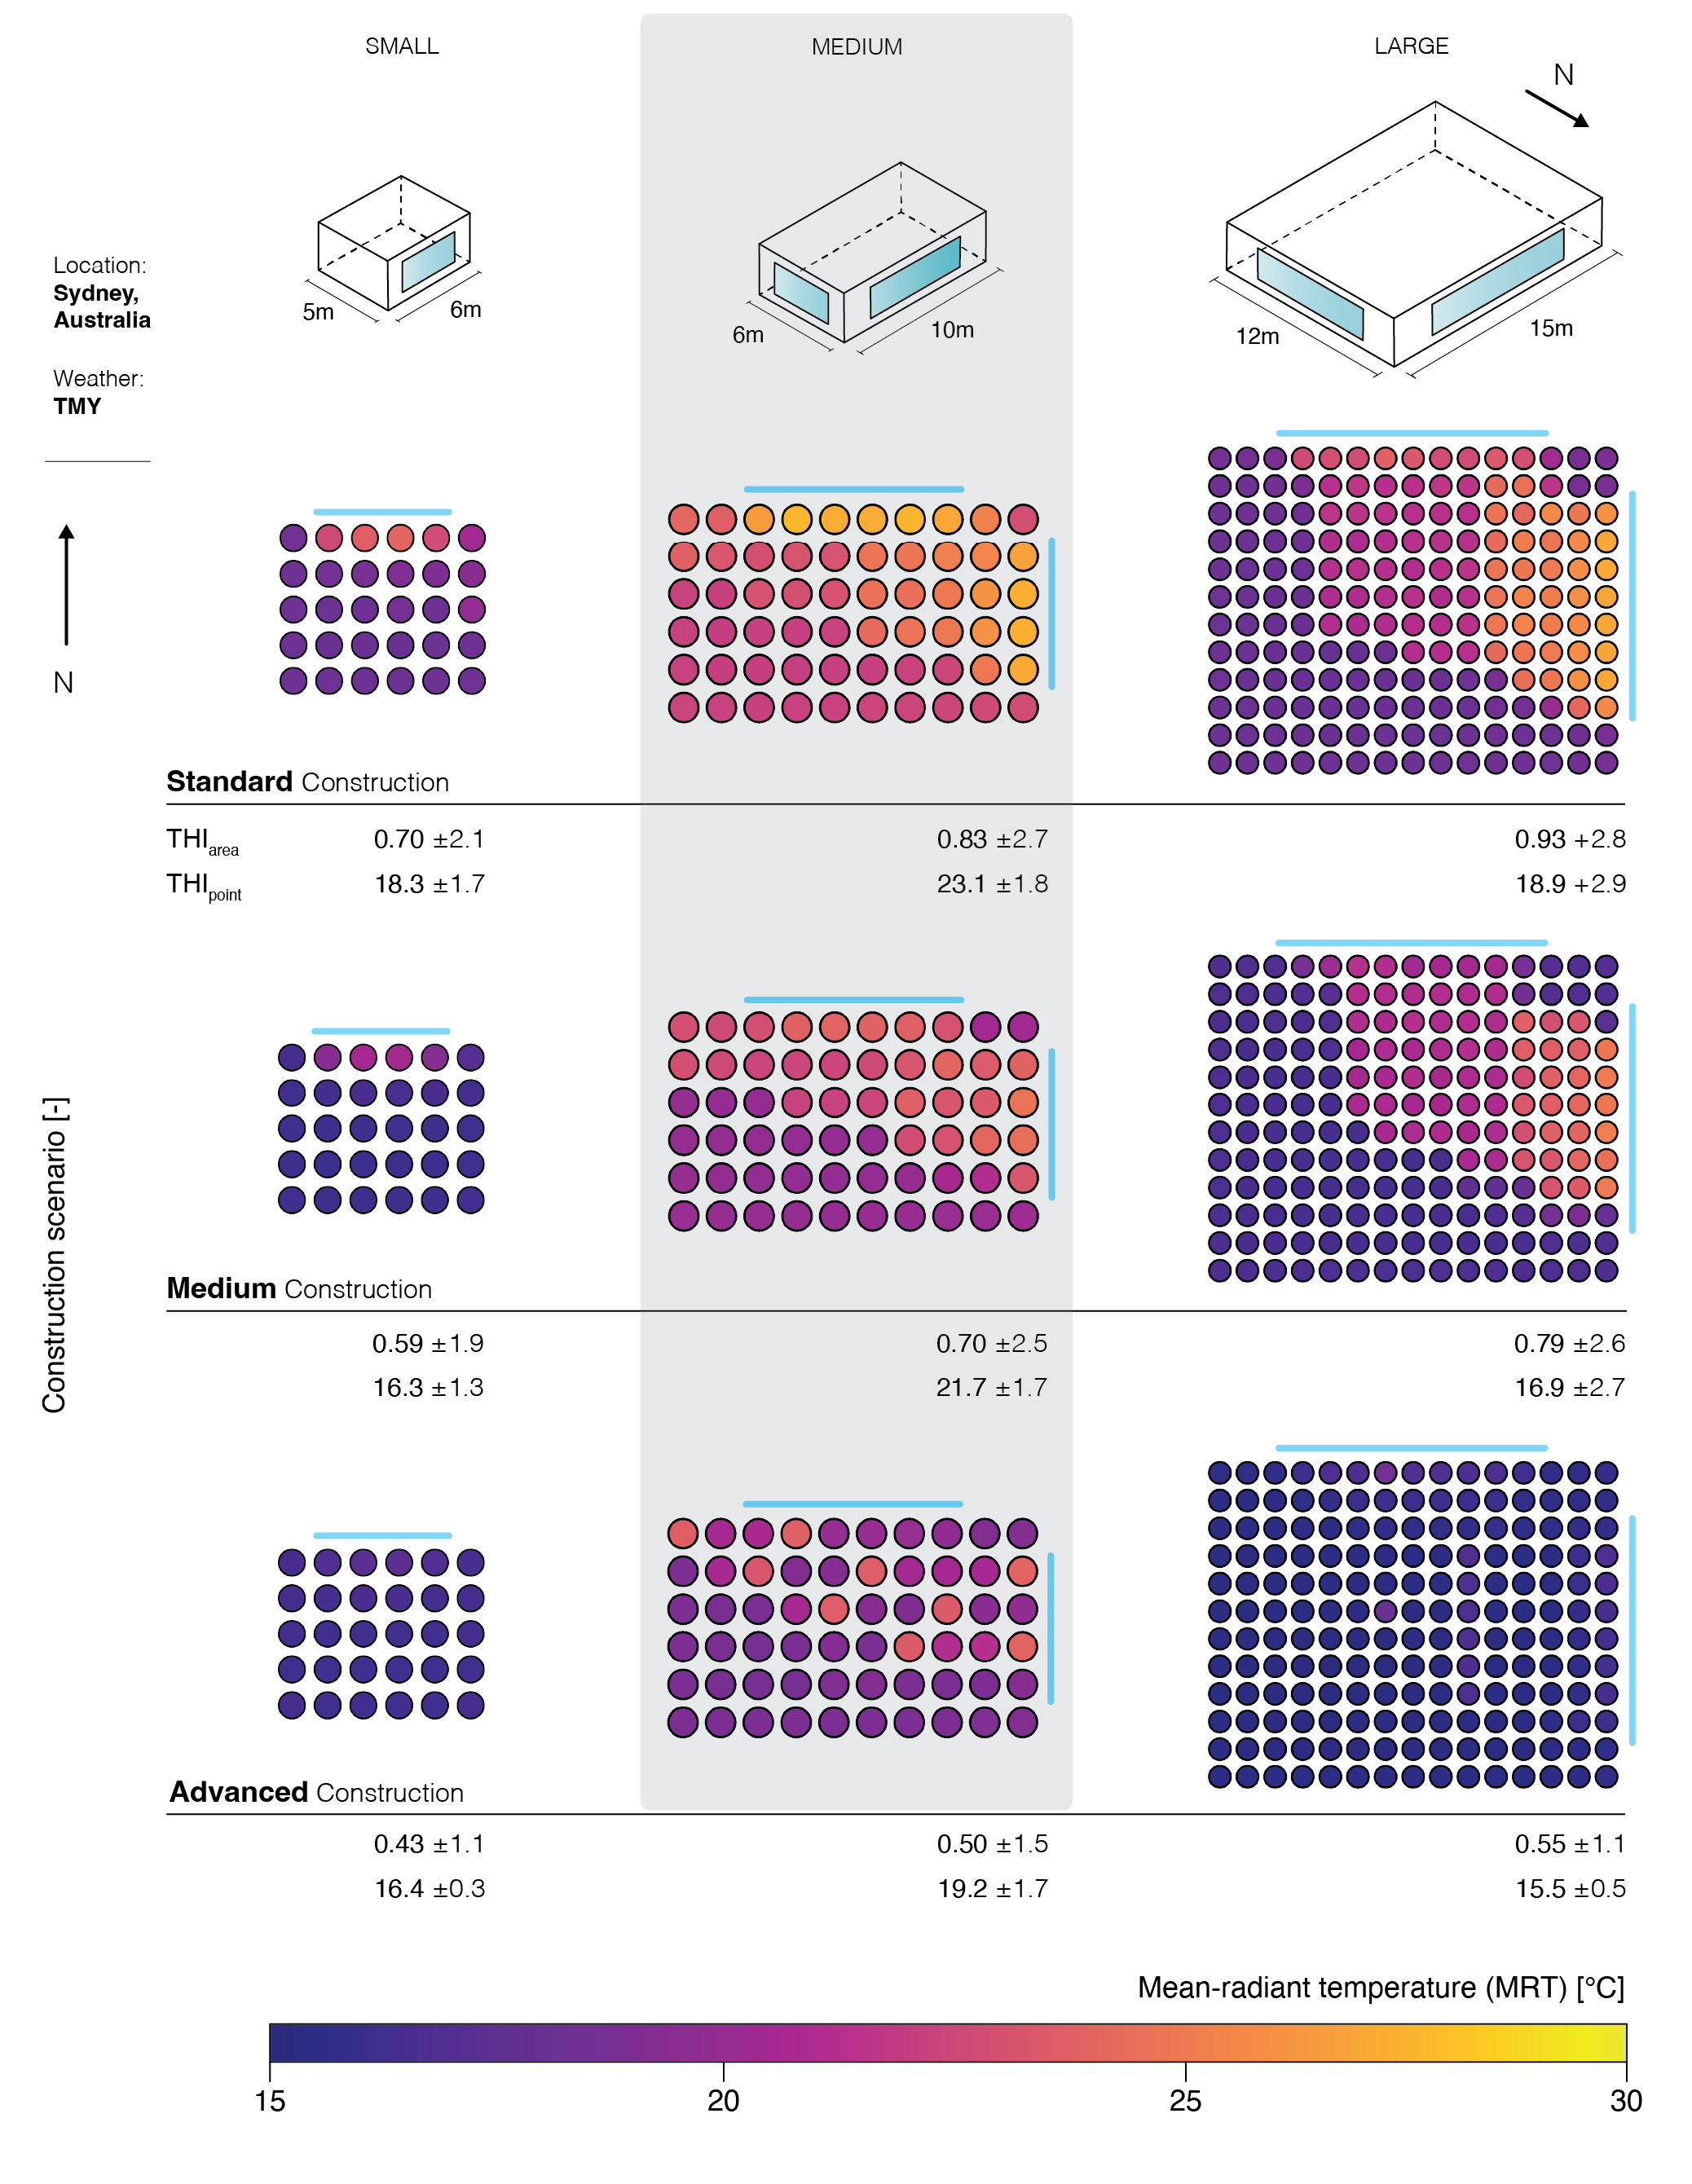
\includegraphics[width=\textwidth]{manuscript/src/figures/heterogeneity-mapping-tmy.png}
    \caption{Annual mean radiant temperature variation and Thermal Heterogeneity Indices (THI) across different zone sizes and construction standards: Mid-sized to larger space show a higher spatial thermal heterogeneity with individual grid-points underlying annual temperature variations of up to 29 °C.}
    \label{fig:heterogeneity-mapping-tmy}
\end{figure}

% ------

In \Cref{fig:zone-mean-v-spatial}, we further explore the variation of indoor temperatures in the thermal zones. Here, we specifically compare the hourly temperature variation across the grid with the conventional standard of only evaluating zone conditions based on a single-point zone mean MRT in the zone center. The results show significant hourly variations between the mean zone MRT and individual grid points, as summarized in the table of percentile distributions in \Cref{fig:zone-mean-v-spatial}. The combined insights from the box plot and table indicate that these deviations are most pronounced in zones with lower construction standards, where the differences between the mean zone MRT and spatial MRT are consistently higher across all percentiles, and in larger spaces, where the plot reveals a considerably wider range of deviations. This reinforces the finding that both zone size and envelope quality play a critical role in moderating thermal conditions.


\begin{figure}[H]
    \centering
    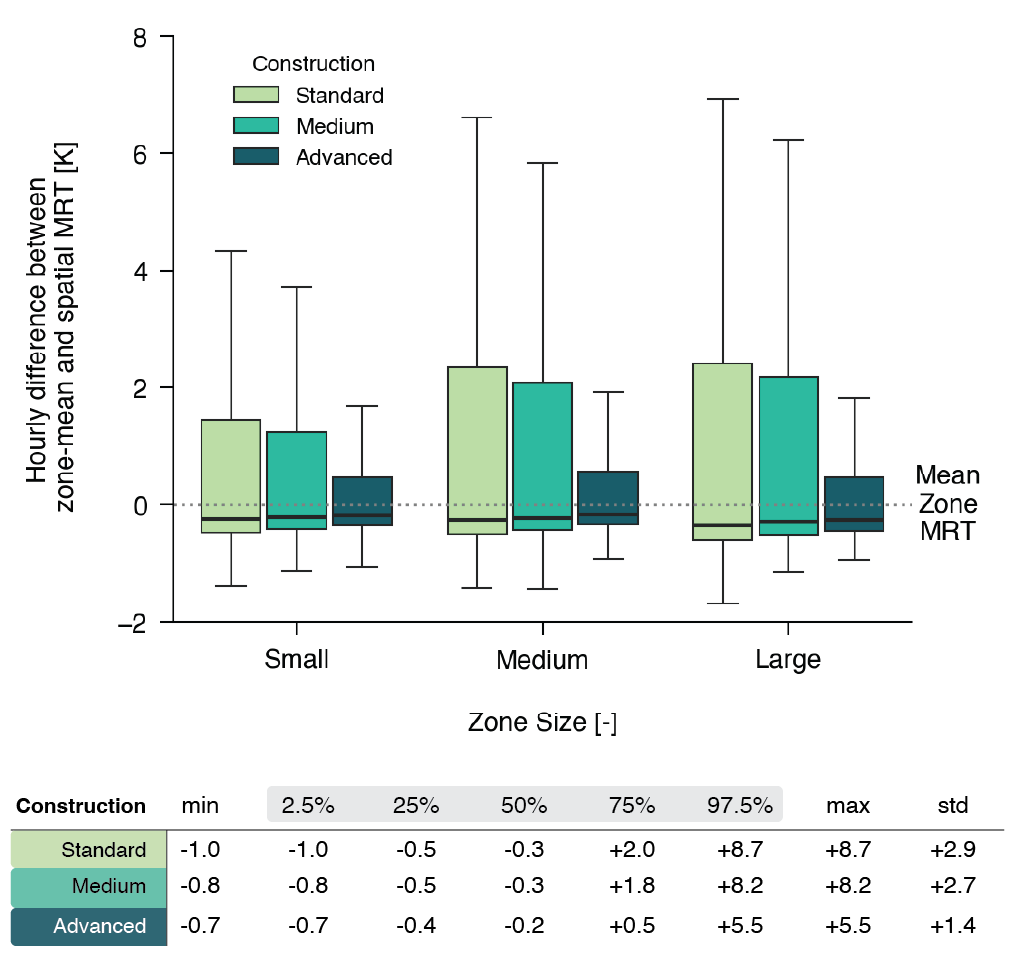
\includegraphics[width=8.9cm]{manuscript/src/figures/zone-mean-v-spatial.png}
    \caption{Distribution of hourly differences between zone-mean MRT and spatially-resolved MRT: Simulating temperature only for the center of the zone (traditional method) overlooks significant thermal fluctuations within the space.}
    \label{fig:zone-mean-v-spatial}
\end{figure}


% sTA, impact of models and area percentage threshold
\subsection{Impact of thermal comfort indices}

In \Cref{fig:model-comparison}.a, we present the distributions of the predicted sTA values hourly using three different thermal comfort indices: PMV, Adaptive, and an Empirical approach based on the ASHRAE Global Thermal Comfort Database II. Across all construction standards tested, the PMV index consistently resulted in the lowest hourly sTA values, with a nearly binary distinction between comfortable and uncomfortable conditions. In contrast, the Adaptive and Empirical models led to generally higher sTA predictions, reflecting a smoother and more gradual transition between low and high hourly sTA values. Moreover, as construction standards improved, we observed an increase in the ratio of higher sTA values, particularly when using the Adaptive and Empirical models. These indices appeared to be more sensitive to changes in envelope performance, capturing the impact of passive design measures more effectively than the PMV index.

\Cref{fig:model-comparison}.b compares the annual sTA values calculated using the three thermal comfort indices, considering different thresholds of the area ratio (see \Cref{eq:sta-annual}). Similarly to the hourly analysis, the PMV index led the lowest annual sTA in all thresholds tested. Only when a low area ratio threshold of 50\% was applied did the sTA values exceed 0.5. In comparison, the adaptive model again consistently predicted higher annual sTA values, independent of construction standards. An improvement in those further enhanced the sTA, with thresholds as high as 80\% still producing sTA values above 0.6, and in the case of high standards, up to 0.8.

The empirical model generated the highest overall sTA values. For the highest construction standards, all area ratio thresholds resulted in sTA values above 0.9, indicating wider comfort ranges and a stronger alignment between passive design and thermal autonomy under this model.

\begin{figure*}[h!]
    \centering
    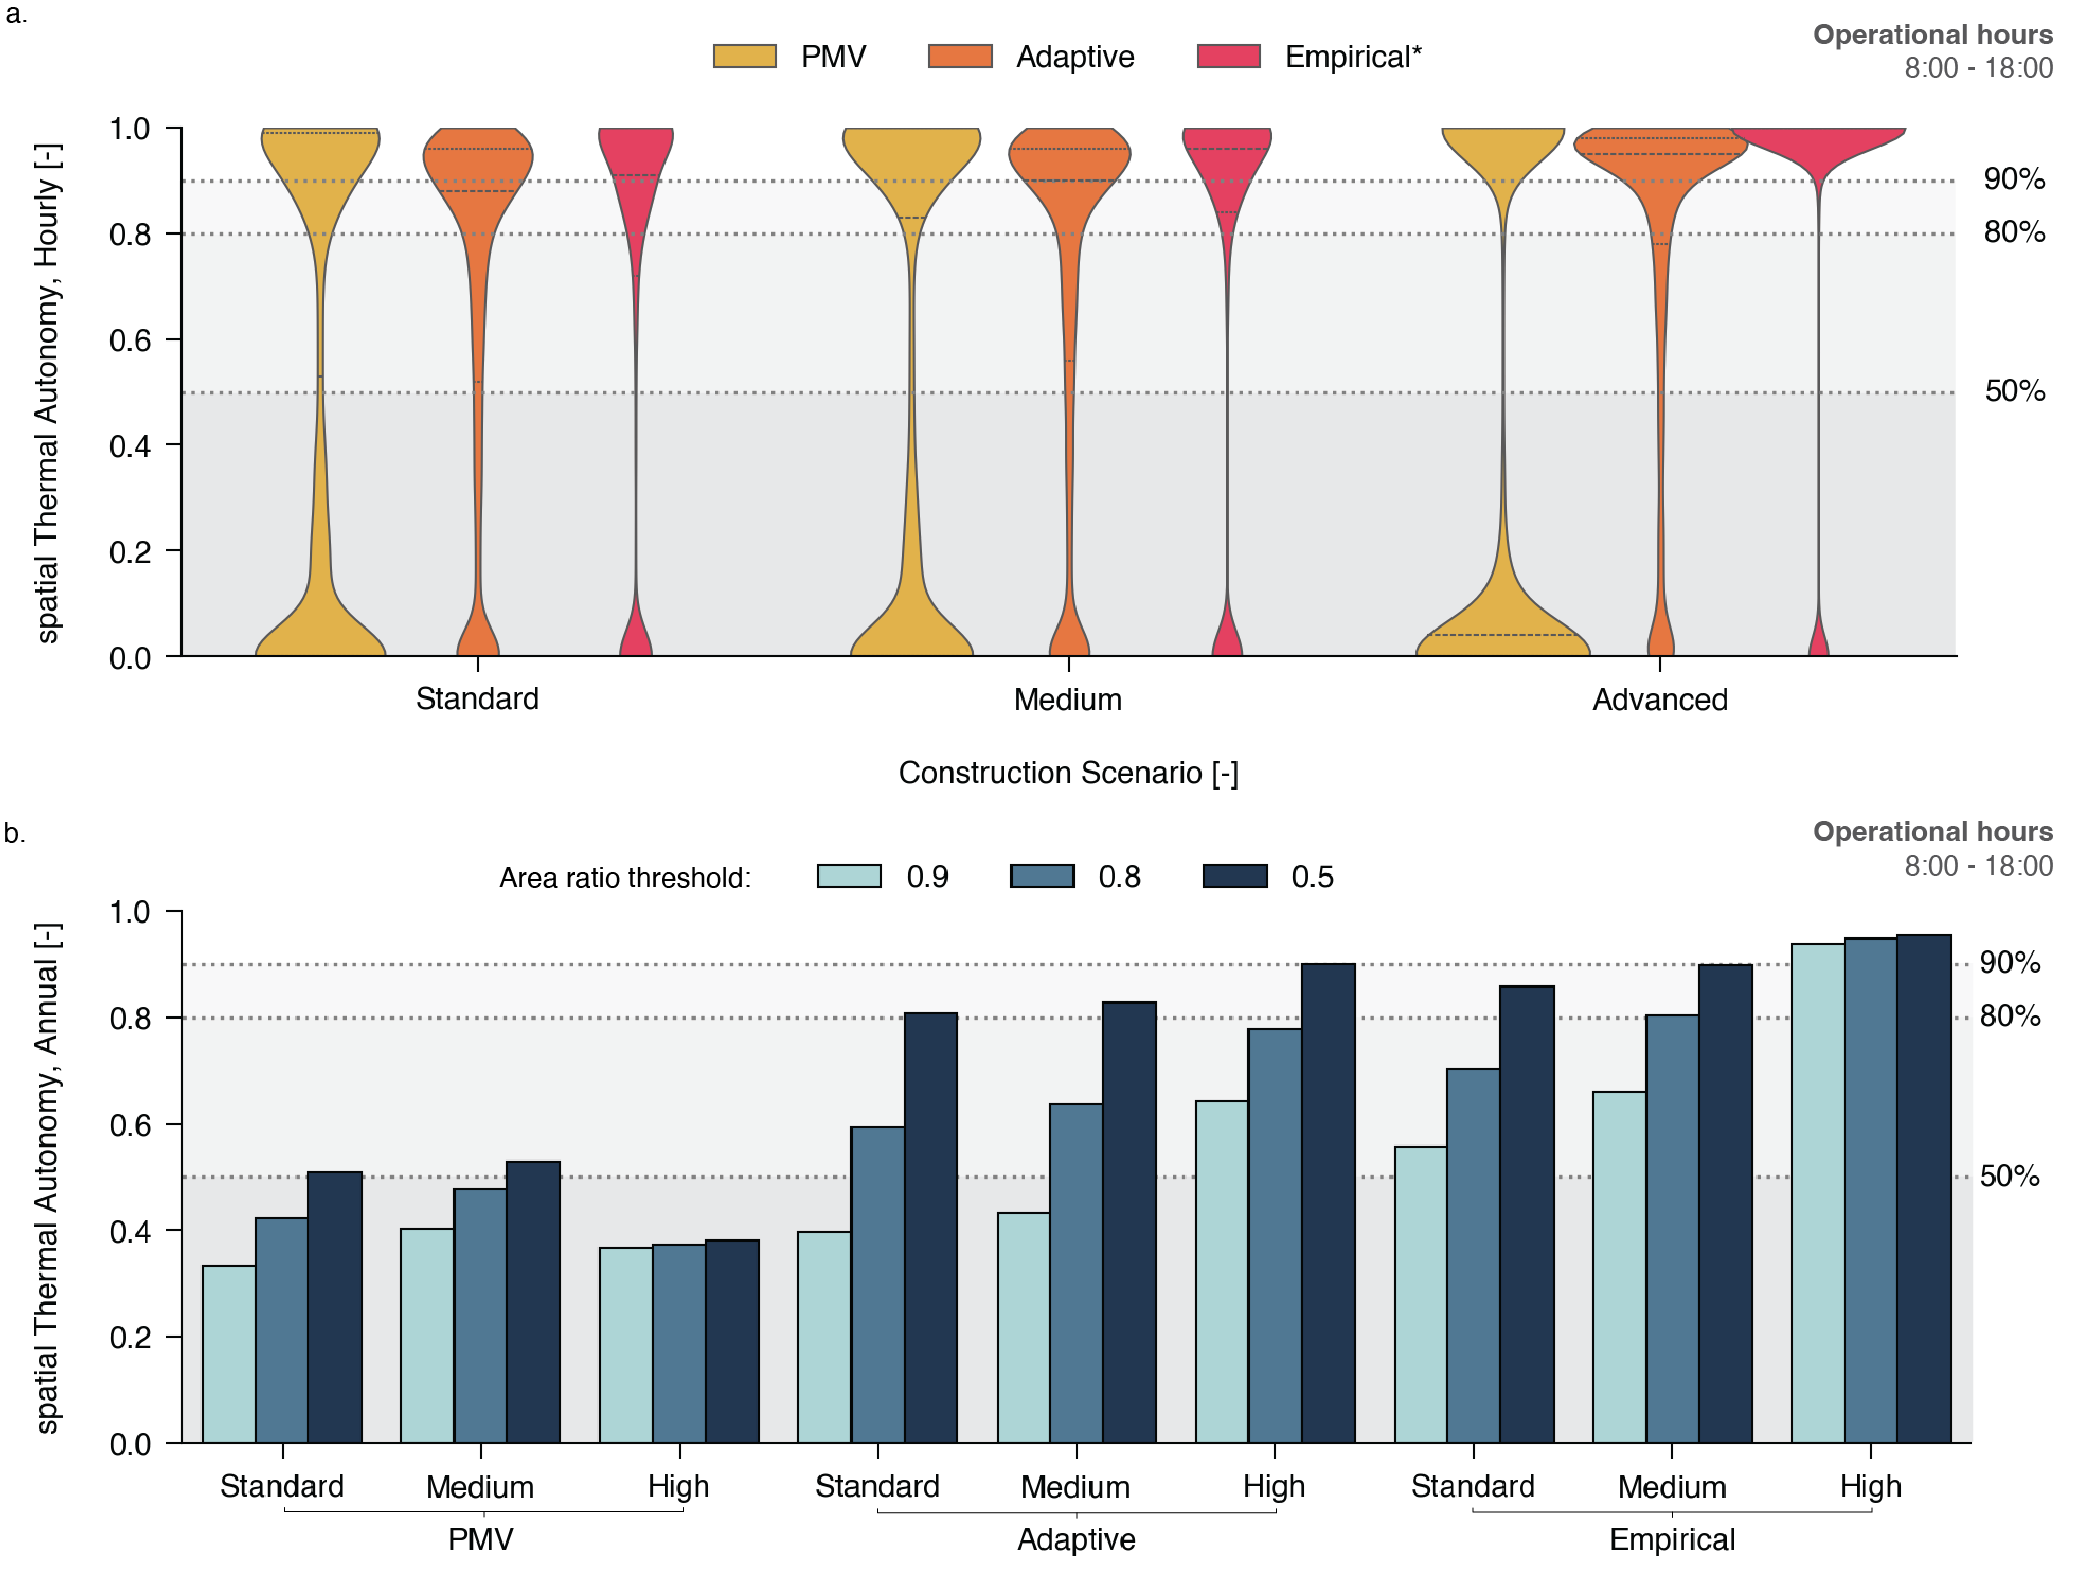
\includegraphics[width=\textwidth]{manuscript/src/figures/model-comparison.png}
    \caption{a) Hourly sTA distributions using PMV, Adaptive, and Empirical models for different passive design levels and medium zone size: Adaptive and Empirical model tend to predict higher sTA$_{hourly}$ and are more sensitive passive design measures; b) Annual sTA comparison across comfort models for varying area ratio thresholds.: Adaptive and Empirical model consistently predict higher sTA$_{annual}$ then PMV, independent of chosen area threshold.}
    \label{fig:model-comparison}
\end{figure*}


% impact on energy use and resilience
\subsection{Energy use and resilience}

\Cref{fig:energy-passive-design}.a illustrates the simulated cooling energy use, averaged across all zone sizes, as a function of construction standards and the two weather scenarios. We observed a significant increase in expected cooling energy demand for the 2070 weather scenario compared to the typical meteorological year (TMY). However, with better construction standards, the computed sTA$_{annual}$ (based on operational hours) also increased, indicating improved thermal performance. Simultaneously, cooling energy use decreased as the construction standard improved, for both the TMY and 2070 scenarios. The reductions were substantial, with a drop of 46\% for TMY and 37\% for the 2070 scenario, underscoring the potential for energy savings through enhanced building envelopes and higher sTA, even in future climate conditions.

In \Cref{fig:energy-passive-design}.b, we compare the passive operative temperature distributions across the simulation grid for each construction standard and the weather scenario. A considerable portion of the operative temperature values exceeded 28 °C, particularly in the 2070 weather and standard construction scenarios. However, as the level of passive design elements improves, the range of operating temperatures narrows, and the proportion of elevated temperatures decreases.

For the advanced construction standard, at least 75\% of the operative temperature values falls below 28 °C for both TMY and 2070, reflecting a significant impact of enhanced passive design on maintaining comfortable indoor conditions, even in future climates, and indicating improved thermal resilience when optimizing sTA.


\begin{figure*}[h!]
    \centering
    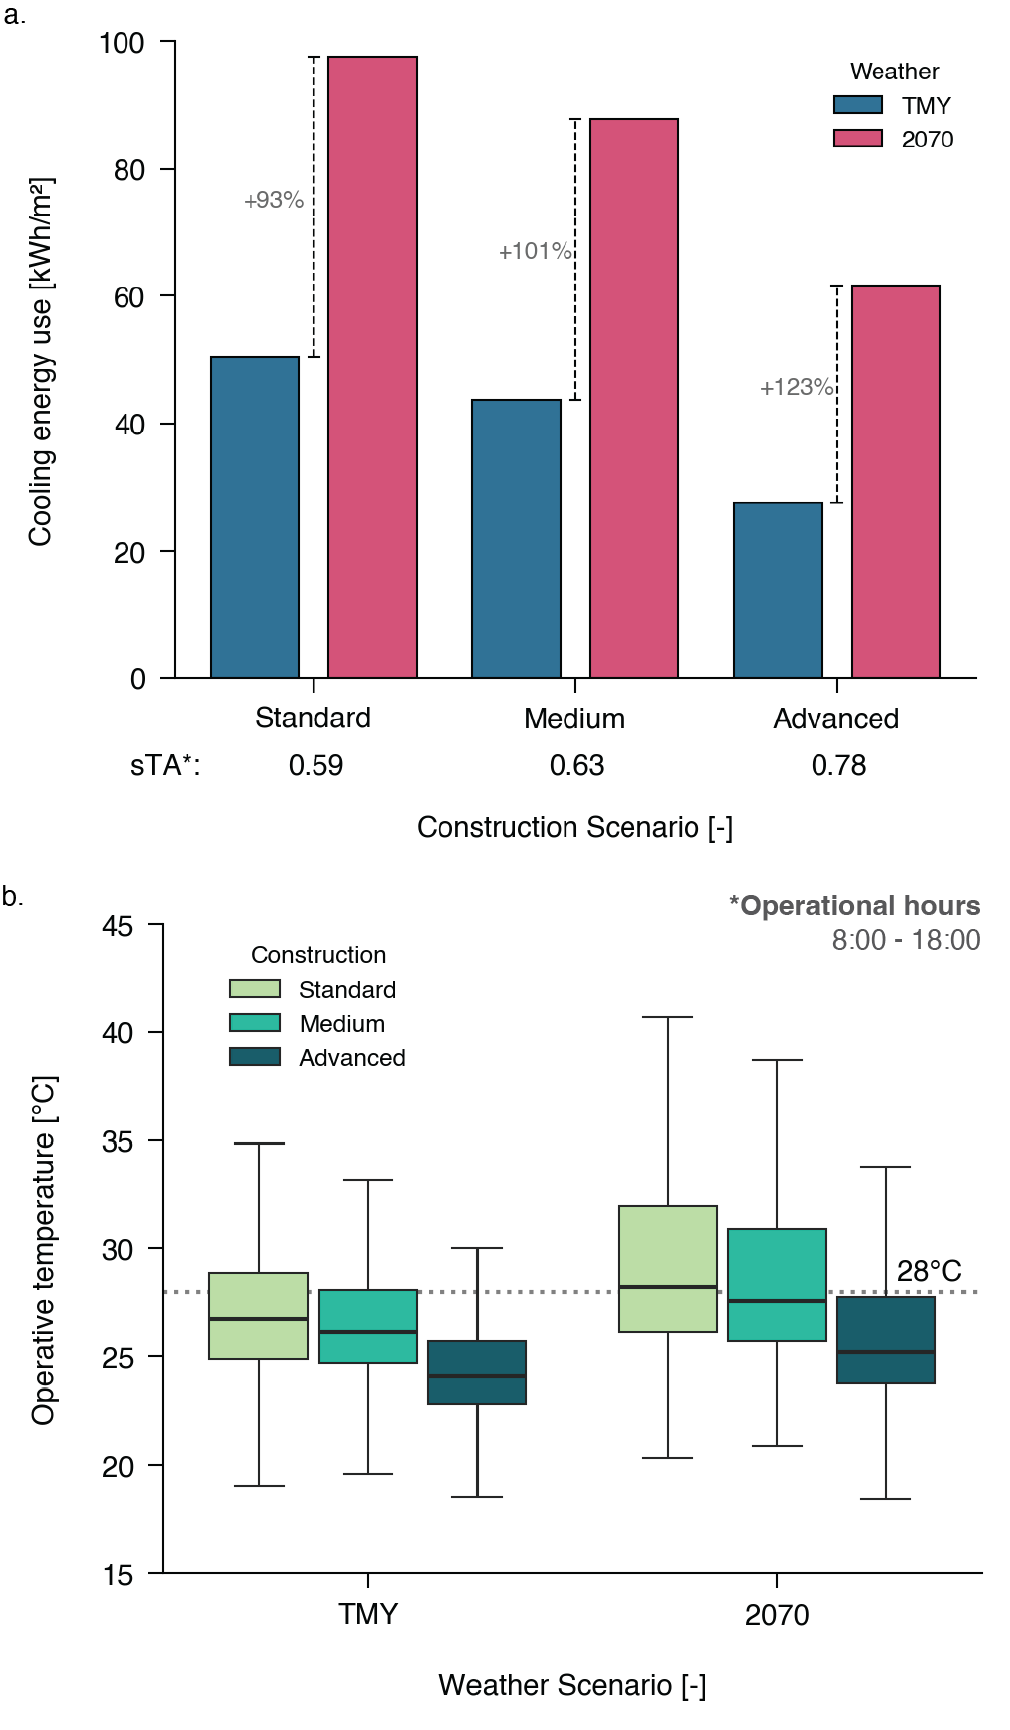
\includegraphics[width=8.9cm]{manuscript/src/figures/energy-passive-design.png}
    \caption{a) Simulated cooling energy use for different construction standards and weather scenarios (Adaptive model, area threshold of 0.8 for sTA$_{annual}$): Higher annual sTA correlates with lower energy use for both TMY and 2070 scenario; b) Passive operative temperature distribution across the grid for different construction standards and weather scenarios.: Higher annual sTA correlates with lower operative temperatures when free-running, indicating higher thermal resilience in both TMY and 2070 scenario.}
    \label{fig:energy-passive-design}
\end{figure*}

Supplementary information, all underlying data and the Python code used for analysis and to generate figures are available on the public \href{https://github.com/t-kramer/2024-paper-conference-cate}{GitHub repository} for this paper.
